\documentclass{whiteboard}
\begin{document}
\begin{frame}[plain,t]
\bbcover{OJ 10308}{Roads in the North}{Prof. Edson Alves}{Faculdade UnB Gama}

\end{frame}
\begin{frame}[plain,t]
\vspace*{\fill}

\bbenglish{Building and maintaining roads among communities in the far North is an expensive business. With this in mind, the roads are built in such a way that there is only one route from a village to a village that does not pass through some other village twice.}

\vspace{0.1in}

\bbenglish{Given is an area in the far North comprising a number of villages and roads among them such that any village can be reached by road from any other village. Your job is to find the road distance between the two most remote villages in the area.}

\vspace{0.1in}

\bbenglish{The area has up to $10,000$ villages connected by road segments. The villages are numbered from $1$.}

\vspace*{\fill}
\end{frame}
\begin{frame}[plain,t]
\vspace*{\fill}

\bbtext{Construir e manter estradas entre comunidades no Norte é um negócio caro. Com isto em mente, as estradas foram construídas de tal modo que há uma única rota entre uma vila e outra e que não passa por uma mesma vila duas vezes.}

\vspace{0.1in}

\bbtext{É dada uma área no Norte composta por um certo número de vilas e estradas que as conectam, de modo que pode-se chegar a qualquer vila a partir de qualquer vila. Seu trabalho é encontrar a distância da rota entre as duas vilas mais remotas desta área.}

\vspace{0.1in}

\bbtext{A área tem no máximo $10.000$ vilas conectadas por estradas. As vilas são numeradas a partir de $1$.}

\vspace*{\fill}
\end{frame}
\begin{frame}[plain,t]
\vspace*{\fill}

\bbbold{Input}

\vspace{0.1in}

\bbenglish{The input contains several sets of input. Each set of input is a sequence of lines, each containing three positive integers: the number of a village, the number of a different village, and the length of the road segment connecting the villages in kilometers. All road segments are two-way. Two consecutive sets are separated by a blank line.}

\vspace{0.2in}

\bbbold{Output}

\vspace{0.1in}

\bbenglish{For each set of input, you are to output a single line containing a single integer: the road distance between the two most remote villages in the area.}

\vspace*{\fill}
\end{frame}
\begin{frame}[plain,t]
\vspace*{\fill}

\bbbold{Entrada}

\vspace{0.1in}

\bbtext{A entrada é composta por vários casos de teste. Cada caso de teste é formado por uma sequência de linhas, cada uma contendo três inteiros positivos: o número de uma vila, o número de uma vila diferente e o comprimento da estrada que conecta estas duas vilas, em kilômetros. Todas as estradas são bidirecionais. Dois casos de teste consecutivos são separados por uma linha em branco.}

\vspace{0.2in}

\bbbold{Saída}

\vspace{0.1in}

\bbtext{Para cada caso de teste, você deve imprimr uma única linha contendo um único inteiro: a distância da rota entre as duas vilas mais remotas da área.}

\vspace*{\fill}
\end{frame}
\begin{frame}[plain,t]
\begin{tikzpicture}
\node[draw,opacity=0] at (0, 0) {x};
\node[draw,opacity=0] at (14, 8) {x};

	\node[anchor=west] (header) at (0, 7.0) { \bbbold{Exemplo de entrada e saída} };

\end{tikzpicture}
\end{frame}
\begin{frame}[plain,t]
\begin{tikzpicture}
\node[draw,opacity=0] at (0, 0) {x};
\node[draw,opacity=0] at (14, 8) {x};

	\node[anchor=west] (header) at (0, 7.0) { \bbbold{Exemplo de entrada e saída} };


	\node[anchor=west] (line1) at (1.0, 6.0) { \bbtext{\texttt{5 1 6} } };

\end{tikzpicture}
\end{frame}
\begin{frame}[plain,t]
\begin{tikzpicture}
\node[draw,opacity=0] at (0, 0) {x};
\node[draw,opacity=0] at (14, 8) {x};

	\node[anchor=west] (header) at (0, 7.0) { \bbbold{Exemplo de entrada e saída} };


	\node[anchor=west] (line1) at (1.0, 6.0) { \bbtext{\texttt{5 1 6} } };


	\draw[->,color=BBViolet] (1.25, 5.0) to  (1.25, 5.75);

	\node[] (r) at (1.25, 4.75) { \footnotesize \bbcomment{vila A} };

\end{tikzpicture}
\end{frame}
\begin{frame}[plain,t]
\begin{tikzpicture}
\node[draw,opacity=0] at (0, 0) {x};
\node[draw,opacity=0] at (14, 8) {x};

	\node[anchor=west] (header) at (0, 7.0) { \bbbold{Exemplo de entrada e saída} };


	\node[anchor=west] (line1) at (1.0, 6.0) { \bbtext{\texttt{5 1 6} } };


	\draw[->,color=BBViolet] (1.65, 5.0) to  (1.65, 5.75);

	\node[] (r) at (1.65, 4.75) { \footnotesize \bbcomment{vila B} };



\end{tikzpicture}
\end{frame}
\begin{frame}[plain,t]
\begin{tikzpicture}
\node[draw,opacity=0] at (0, 0) {x};
\node[draw,opacity=0] at (14, 8) {x};

	\node[anchor=west] (header) at (0, 7.0) { \bbbold{Exemplo de entrada e saída} };


	\node[anchor=west] (line1) at (1.0, 6.0) { \bbtext{\texttt{5 1 6} } };


	\draw[->,color=BBViolet] (2.05, 5.0) to  (2.05, 5.75);

	\node[] (r) at (2.05, 4.75) { \footnotesize \bbcomment{distância entre A e B} };





\end{tikzpicture}
\end{frame}
\begin{frame}[plain,t]
\begin{tikzpicture}
\node[draw,opacity=0] at (0, 0) {x};
\node[draw,opacity=0] at (14, 8) {x};

	\node[anchor=west] (header) at (0, 7.0) { \bbbold{Exemplo de entrada e saída} };


	\node[anchor=west] (line1) at (1.0, 6.0) { \bbtext{\texttt{5 1 6} } };










	\node[draw,very thick,circle] (node1) at (7.0, 5.0) { \bbtext{1} };




	\node[draw,very thick,circle] (node5) at (10.0, 1.0) { \bbtext{5} };



	\draw[thick](node5) to node[above right,pos=0.2] { \bbinfo{6} } (node1);

\end{tikzpicture}
\end{frame}
\begin{frame}[plain,t]
\begin{tikzpicture}
\node[draw,opacity=0] at (0, 0) {x};
\node[draw,opacity=0] at (14, 8) {x};

	\node[anchor=west] (header) at (0, 7.0) { \bbbold{Exemplo de entrada e saída} };


	\node[anchor=west] (line1) at (1.0, 6.0) { \bbtext{\texttt{5 1 6} } };










	\node[draw,very thick,circle] (node1) at (7.0, 5.0) { \bbtext{1} };




	\node[draw,very thick,circle] (node5) at (10.0, 1.0) { \bbtext{5} };



	\draw[thick](node5) to node[above right,pos=0.2] { \bbinfo{6} } (node1);


	\node[anchor=west] (line2) at (1.0, 5.5) { \bbtext{\texttt{1 4 5} } };

\end{tikzpicture}
\end{frame}
\begin{frame}[plain,t]
\begin{tikzpicture}
\node[draw,opacity=0] at (0, 0) {x};
\node[draw,opacity=0] at (14, 8) {x};

	\node[anchor=west] (header) at (0, 7.0) { \bbbold{Exemplo de entrada e saída} };


	\node[anchor=west] (line1) at (1.0, 6.0) { \bbtext{\texttt{5 1 6} } };










	\node[draw,very thick,circle] (node1) at (7.0, 5.0) { \bbtext{1} };



	\node[draw,very thick,circle] (node4) at (13.0, 3.0) { \bbtext{4} };

	\node[draw,very thick,circle] (node5) at (10.0, 1.0) { \bbtext{5} };



	\draw[thick](node5) to node[above right,pos=0.2] { \bbinfo{6} } (node1);


	\node[anchor=west] (line2) at (1.0, 5.5) { \bbtext{\texttt{1 4 5} } };



	\draw[thick](node4) to node[above right,pos=0.7] { \bbinfo{5} } (node1);


\end{tikzpicture}
\end{frame}
\begin{frame}[plain,t]
\begin{tikzpicture}
\node[draw,opacity=0] at (0, 0) {x};
\node[draw,opacity=0] at (14, 8) {x};

	\node[anchor=west] (header) at (0, 7.0) { \bbbold{Exemplo de entrada e saída} };


	\node[anchor=west] (line1) at (1.0, 6.0) { \bbtext{\texttt{5 1 6} } };










	\node[draw,very thick,circle] (node1) at (7.0, 5.0) { \bbtext{1} };



	\node[draw,very thick,circle] (node4) at (13.0, 3.0) { \bbtext{4} };

	\node[draw,very thick,circle] (node5) at (10.0, 1.0) { \bbtext{5} };



	\draw[thick](node5) to node[above right,pos=0.2] { \bbinfo{6} } (node1);


	\node[anchor=west] (line2) at (1.0, 5.5) { \bbtext{\texttt{1 4 5} } };



	\draw[thick](node4) to node[above right,pos=0.7] { \bbinfo{5} } (node1);



	\node[anchor=west] (line3) at (1.0, 5.0) { \bbtext{\texttt{6 3 9} } };

\end{tikzpicture}
\end{frame}
\begin{frame}[plain,t]
\begin{tikzpicture}
\node[draw,opacity=0] at (0, 0) {x};
\node[draw,opacity=0] at (14, 8) {x};

	\node[anchor=west] (header) at (0, 7.0) { \bbbold{Exemplo de entrada e saída} };


	\node[anchor=west] (line1) at (1.0, 6.0) { \bbtext{\texttt{5 1 6} } };










	\node[draw,very thick,circle] (node1) at (7.0, 5.0) { \bbtext{1} };


	\node[draw,very thick,circle] (node3) at (13.0, 5.0) { \bbtext{3} };

	\node[draw,very thick,circle] (node4) at (13.0, 3.0) { \bbtext{4} };

	\node[draw,very thick,circle] (node5) at (10.0, 1.0) { \bbtext{5} };

	\node[draw,very thick,circle] (node6) at (7.0, 3.0) { \bbtext{6} };


	\draw[thick](node5) to node[above right,pos=0.2] { \bbinfo{6} } (node1);


	\node[anchor=west] (line2) at (1.0, 5.5) { \bbtext{\texttt{1 4 5} } };



	\draw[thick](node4) to node[above right,pos=0.7] { \bbinfo{5} } (node1);



	\node[anchor=west] (line3) at (1.0, 5.0) { \bbtext{\texttt{6 3 9} } };


	\draw[thick](node6) to node[above right,pos=0.7] { \bbinfo{9} } (node3);

\end{tikzpicture}
\end{frame}
\begin{frame}[plain,t]
\begin{tikzpicture}
\node[draw,opacity=0] at (0, 0) {x};
\node[draw,opacity=0] at (14, 8) {x};

	\node[anchor=west] (header) at (0, 7.0) { \bbbold{Exemplo de entrada e saída} };


	\node[anchor=west] (line1) at (1.0, 6.0) { \bbtext{\texttt{5 1 6} } };










	\node[draw,very thick,circle] (node1) at (7.0, 5.0) { \bbtext{1} };


	\node[draw,very thick,circle] (node3) at (13.0, 5.0) { \bbtext{3} };

	\node[draw,very thick,circle] (node4) at (13.0, 3.0) { \bbtext{4} };

	\node[draw,very thick,circle] (node5) at (10.0, 1.0) { \bbtext{5} };

	\node[draw,very thick,circle] (node6) at (7.0, 3.0) { \bbtext{6} };


	\draw[thick](node5) to node[above right,pos=0.2] { \bbinfo{6} } (node1);


	\node[anchor=west] (line2) at (1.0, 5.5) { \bbtext{\texttt{1 4 5} } };



	\draw[thick](node4) to node[above right,pos=0.7] { \bbinfo{5} } (node1);



	\node[anchor=west] (line3) at (1.0, 5.0) { \bbtext{\texttt{6 3 9} } };


	\draw[thick](node6) to node[above right,pos=0.7] { \bbinfo{9} } (node3);


	\node[anchor=west] (line4) at (1.0, 4.5) { \bbtext{\texttt{2 6 8} } };

\end{tikzpicture}
\end{frame}
\begin{frame}[plain,t]
\begin{tikzpicture}
\node[draw,opacity=0] at (0, 0) {x};
\node[draw,opacity=0] at (14, 8) {x};

	\node[anchor=west] (header) at (0, 7.0) { \bbbold{Exemplo de entrada e saída} };


	\node[anchor=west] (line1) at (1.0, 6.0) { \bbtext{\texttt{5 1 6} } };










	\node[draw,very thick,circle] (node1) at (7.0, 5.0) { \bbtext{1} };

	\node[draw,very thick,circle] (node2) at (10.0, 7.0) { \bbtext{2} };

	\node[draw,very thick,circle] (node3) at (13.0, 5.0) { \bbtext{3} };

	\node[draw,very thick,circle] (node4) at (13.0, 3.0) { \bbtext{4} };

	\node[draw,very thick,circle] (node5) at (10.0, 1.0) { \bbtext{5} };

	\node[draw,very thick,circle] (node6) at (7.0, 3.0) { \bbtext{6} };


	\draw[thick](node5) to node[above right,pos=0.2] { \bbinfo{6} } (node1);


	\node[anchor=west] (line2) at (1.0, 5.5) { \bbtext{\texttt{1 4 5} } };



	\draw[thick](node4) to node[above right,pos=0.7] { \bbinfo{5} } (node1);



	\node[anchor=west] (line3) at (1.0, 5.0) { \bbtext{\texttt{6 3 9} } };


	\draw[thick](node6) to node[above right,pos=0.7] { \bbinfo{9} } (node3);


	\node[anchor=west] (line4) at (1.0, 4.5) { \bbtext{\texttt{2 6 8} } };


	\draw[thick](node6) to node[above left,pos=0.7] { \bbinfo{8} } (node2);

\end{tikzpicture}
\end{frame}
\begin{frame}[plain,t]
\begin{tikzpicture}
\node[draw,opacity=0] at (0, 0) {x};
\node[draw,opacity=0] at (14, 8) {x};

	\node[anchor=west] (header) at (0, 7.0) { \bbbold{Exemplo de entrada e saída} };


	\node[anchor=west] (line1) at (1.0, 6.0) { \bbtext{\texttt{5 1 6} } };










	\node[draw,very thick,circle] (node1) at (7.0, 5.0) { \bbtext{1} };

	\node[draw,very thick,circle] (node2) at (10.0, 7.0) { \bbtext{2} };

	\node[draw,very thick,circle] (node3) at (13.0, 5.0) { \bbtext{3} };

	\node[draw,very thick,circle] (node4) at (13.0, 3.0) { \bbtext{4} };

	\node[draw,very thick,circle] (node5) at (10.0, 1.0) { \bbtext{5} };

	\node[draw,very thick,circle] (node6) at (7.0, 3.0) { \bbtext{6} };


	\draw[thick](node5) to node[above right,pos=0.2] { \bbinfo{6} } (node1);


	\node[anchor=west] (line2) at (1.0, 5.5) { \bbtext{\texttt{1 4 5} } };



	\draw[thick](node4) to node[above right,pos=0.7] { \bbinfo{5} } (node1);



	\node[anchor=west] (line3) at (1.0, 5.0) { \bbtext{\texttt{6 3 9} } };


	\draw[thick](node6) to node[above right,pos=0.7] { \bbinfo{9} } (node3);


	\node[anchor=west] (line4) at (1.0, 4.5) { \bbtext{\texttt{2 6 8} } };


	\draw[thick](node6) to node[above left,pos=0.7] { \bbinfo{8} } (node2);


	\node[anchor=west] (line5) at (1.0, 4.0) { \bbtext{\texttt{6 1 7} } };

\end{tikzpicture}
\end{frame}
\begin{frame}[plain,t]
\begin{tikzpicture}
\node[draw,opacity=0] at (0, 0) {x};
\node[draw,opacity=0] at (14, 8) {x};

	\node[anchor=west] (header) at (0, 7.0) { \bbbold{Exemplo de entrada e saída} };


	\node[anchor=west] (line1) at (1.0, 6.0) { \bbtext{\texttt{5 1 6} } };










	\node[draw,very thick,circle] (node1) at (7.0, 5.0) { \bbtext{1} };

	\node[draw,very thick,circle] (node2) at (10.0, 7.0) { \bbtext{2} };

	\node[draw,very thick,circle] (node3) at (13.0, 5.0) { \bbtext{3} };

	\node[draw,very thick,circle] (node4) at (13.0, 3.0) { \bbtext{4} };

	\node[draw,very thick,circle] (node5) at (10.0, 1.0) { \bbtext{5} };

	\node[draw,very thick,circle] (node6) at (7.0, 3.0) { \bbtext{6} };


	\draw[thick](node5) to node[above right,pos=0.2] { \bbinfo{6} } (node1);


	\node[anchor=west] (line2) at (1.0, 5.5) { \bbtext{\texttt{1 4 5} } };



	\draw[thick](node4) to node[above right,pos=0.7] { \bbinfo{5} } (node1);



	\node[anchor=west] (line3) at (1.0, 5.0) { \bbtext{\texttt{6 3 9} } };


	\draw[thick](node6) to node[above right,pos=0.7] { \bbinfo{9} } (node3);


	\node[anchor=west] (line4) at (1.0, 4.5) { \bbtext{\texttt{2 6 8} } };


	\draw[thick](node6) to node[above left,pos=0.7] { \bbinfo{8} } (node2);


	\node[anchor=west] (line5) at (1.0, 4.0) { \bbtext{\texttt{6 1 7} } };


	\draw[thick](node6) to node[left] { \bbinfo{7} } (node1);

\end{tikzpicture}
\end{frame}
\begin{frame}[plain,t]
\begin{tikzpicture}
\node[draw,opacity=0] at (0, 0) {x};
\node[draw,opacity=0] at (14, 8) {x};

	\node[anchor=west] (header) at (0, 7.0) { \bbbold{Exemplo de entrada e saída} };


	\node[anchor=west] (line1) at (1.0, 6.0) { \bbtext{\texttt{5 1 6} } };










	\node[draw,very thick,circle] (node1) at (7.0, 5.0) { \bbtext{1} };

	\node[draw,very thick,circle] (node2) at (10.0, 7.0) { \bbtext{2} };

	\node[draw,very thick,circle] (node3) at (13.0, 5.0) { \bbtext{3} };

	\node[draw,very thick,circle] (node4) at (13.0, 3.0) { \bbtext{4} };

	\node[draw,very thick,circle] (node5) at (10.0, 1.0) { \bbtext{5} };

	\node[draw,very thick,circle] (node6) at (7.0, 3.0) { \bbtext{6} };


	\draw[thick,color=BBCyan,dashed](node5) to node[above right,pos=0.2] { \bbinfo{6} } (node1);


	\node[anchor=west] (line2) at (1.0, 5.5) { \bbtext{\texttt{1 4 5} } };



	\draw[thick](node4) to node[above right,pos=0.7] { \bbinfo{5} } (node1);



	\node[anchor=west] (line3) at (1.0, 5.0) { \bbtext{\texttt{6 3 9} } };


	\draw[thick,color=BBCyan,dashed](node6) to node[above right,pos=0.7] { \bbinfo{9} } (node3);


	\node[anchor=west] (line4) at (1.0, 4.5) { \bbtext{\texttt{2 6 8} } };


	\draw[thick](node6) to node[above left,pos=0.7] { \bbinfo{8} } (node2);


	\node[anchor=west] (line5) at (1.0, 4.0) { \bbtext{\texttt{6 1 7} } };


	\draw[thick,color=BBCyan,dashed](node6) to node[left] { \bbinfo{7} } (node1);





\end{tikzpicture}
\end{frame}
\begin{frame}[plain,t]
\begin{tikzpicture}
\node[draw,opacity=0] at (0, 0) {x};
\node[draw,opacity=0] at (14, 8) {x};

	\node[anchor=west] (header) at (0, 7.0) { \bbbold{Exemplo de entrada e saída} };


	\node[anchor=west] (line1) at (1.0, 6.0) { \bbtext{\texttt{5 1 6} } };


	\draw[->,color=BBBlack,very thick,-latex] (1.65, 2.75) to  (1.65, 3.75);

	\node[] (r) at (1.65, 2.5) { \bboutput{6 + 7 + 9 = 22} };







	\node[draw,very thick,circle] (node1) at (7.0, 5.0) { \bbtext{1} };

	\node[draw,very thick,circle] (node2) at (10.0, 7.0) { \bbtext{2} };

	\node[draw,very thick,circle] (node3) at (13.0, 5.0) { \bbtext{3} };

	\node[draw,very thick,circle] (node4) at (13.0, 3.0) { \bbtext{4} };

	\node[draw,very thick,circle] (node5) at (10.0, 1.0) { \bbtext{5} };

	\node[draw,very thick,circle] (node6) at (7.0, 3.0) { \bbtext{6} };


	\draw[thick,color=BBCyan,dashed](node5) to node[above right,pos=0.2] { \bbinfo{6} } (node1);


	\node[anchor=west] (line2) at (1.0, 5.5) { \bbtext{\texttt{1 4 5} } };



	\draw[thick](node4) to node[above right,pos=0.7] { \bbinfo{5} } (node1);



	\node[anchor=west] (line3) at (1.0, 5.0) { \bbtext{\texttt{6 3 9} } };


	\draw[thick,color=BBCyan,dashed](node6) to node[above right,pos=0.7] { \bbinfo{9} } (node3);


	\node[anchor=west] (line4) at (1.0, 4.5) { \bbtext{\texttt{2 6 8} } };


	\draw[thick](node6) to node[above left,pos=0.7] { \bbinfo{8} } (node2);


	\node[anchor=west] (line5) at (1.0, 4.0) { \bbtext{\texttt{6 1 7} } };


	\draw[thick,color=BBCyan,dashed](node6) to node[left] { \bbinfo{7} } (node1);








\end{tikzpicture}
\end{frame}
\begin{frame}[plain,t]
\begin{tikzpicture}
\node[draw,opacity=0] at (0, 0) {x};
\node[draw,opacity=0] at (14, 8) {x};

	\node[anchor=west] (header) at (0.0, 6.0) { \Large \bbbold{Solução} };

\end{tikzpicture}
\end{frame}
\begin{frame}[plain,t]
\begin{tikzpicture}
\node[draw,opacity=0] at (0, 0) {x};
\node[draw,opacity=0] at (14, 8) {x};

	\node[anchor=west] (header) at (0.0, 6.0) { \Large \bbbold{Solução} };


	\node[anchor=west] (a) at (1.0, 5.0) { $\star$ \bbtext{As vilas mais remotas são as mais distantes entre si} };

\end{tikzpicture}
\end{frame}
\begin{frame}[plain,t]
\begin{tikzpicture}
\node[draw,opacity=0] at (0, 0) {x};
\node[draw,opacity=0] at (14, 8) {x};

	\node[anchor=west] (header) at (0.0, 6.0) { \Large \bbbold{Solução} };


	\node[anchor=west] (a) at (1.0, 5.0) { $\star$ \bbtext{As vilas mais remotas são as mais distantes entre si} };


	\node[anchor=west] (b) at (1.0, 4.0) { $\star$ \bbtext{Neste problema, as vilas são os vértices e as estradas são arestas} };

\end{tikzpicture}
\end{frame}
\begin{frame}[plain,t]
\begin{tikzpicture}
\node[draw,opacity=0] at (0, 0) {x};
\node[draw,opacity=0] at (14, 8) {x};

	\node[anchor=west] (header) at (0.0, 6.0) { \Large \bbbold{Solução} };


	\node[anchor=west] (a) at (1.0, 5.0) { $\star$ \bbtext{As vilas mais remotas são as mais distantes entre si} };


	\node[anchor=west] (b) at (1.0, 4.0) { $\star$ \bbtext{Neste problema, as vilas são os vértices e as estradas são arestas} };


	\node[anchor=west] (c) at (1.0, 3.0) { $\star$ \bbtext{As características dadas no texto tornam o grafo uma árvore} };

\end{tikzpicture}
\end{frame}
\begin{frame}[plain,t]
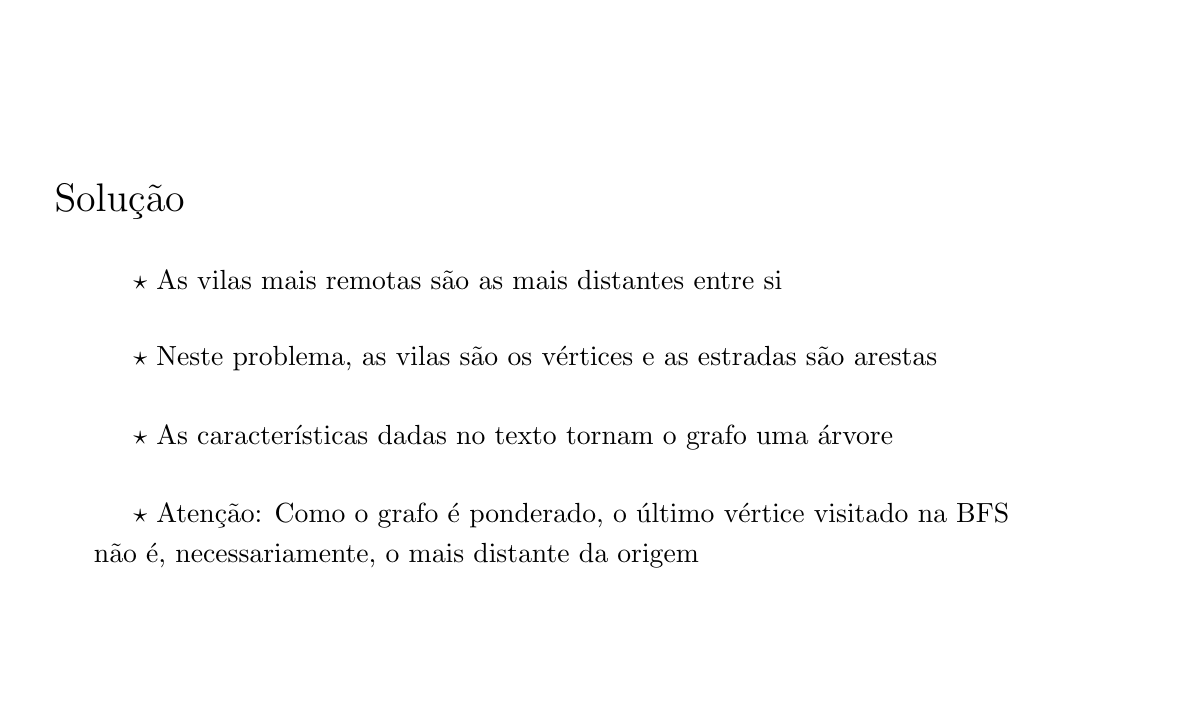
\begin{tikzpicture}
\node[draw,opacity=0] at (0, 0) {x};
\node[draw,opacity=0] at (14, 8) {x};

	\node[anchor=west] (header) at (0.0, 6.0) { \Large \bbbold{Solução} };


	\node[anchor=west] (a) at (1.0, 5.0) { $\star$ \bbtext{As vilas mais remotas são as mais distantes entre si} };


	\node[anchor=west] (b) at (1.0, 4.0) { $\star$ \bbtext{Neste problema, as vilas são os vértices e as estradas são arestas} };


	\node[anchor=west] (c) at (1.0, 3.0) { $\star$ \bbtext{As características dadas no texto tornam o grafo uma árvore} };


	\node[anchor=west] (d) at (1.0, 2.0) { $\star$ \bbbold{Atenção:} \bbtext{Como o grafo é ponderado, o último vértice visitado na BFS} };

	\node[anchor=west] (d1) at (0.5, 1.5) { \bbtext{não é, necessariamente, o mais distante da origem} };

\end{tikzpicture}
\end{frame}
\begin{frame}[plain,t]

\inputsnippet{cpp}{9}{28}{codes/10308.cpp}

\end{frame}
\begin{frame}[plain,t]

\inputsnippet{cpp}{30}{43}{codes/10308.cpp}

\end{frame}
\end{document}
